\section{Problem 1 - Simulations with NETLOGO}
Install the program and do the following. (http://ccl.northwestern.edu/netlogo/)
\subsection{Compare the revenue for 10 TIT-FOR-TAT and 10 DEFECT turtles}

The simulation is setup in the software and the resulting plot is shown in \figref{fig:10tft_10def-jpg}.
\begin{figure}[!h]
  \centering
  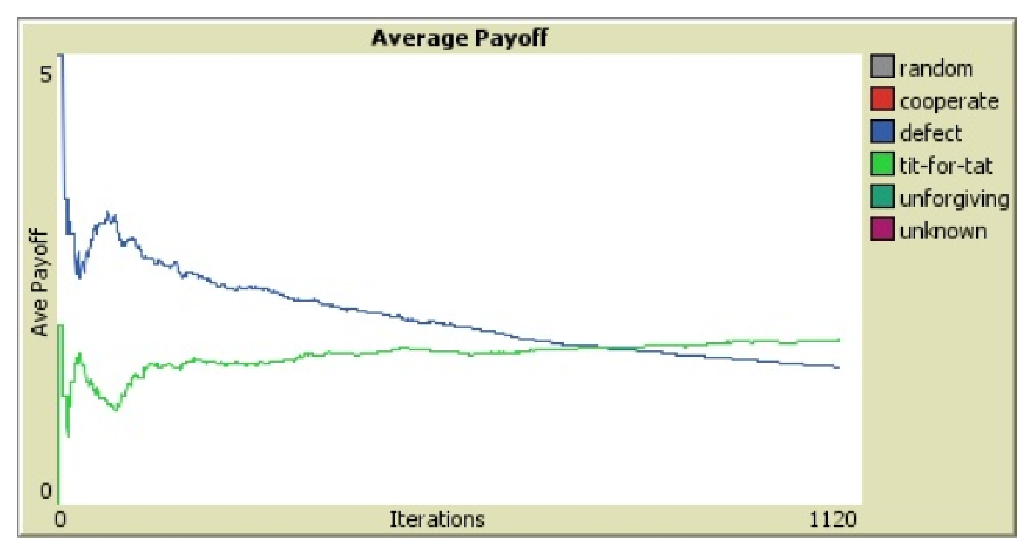
\includegraphics[width=10cm]{10tft_10def-jpg.eps}
  \caption{Simulation for 10 TIT-FOR-TAT and 10 DEFECT turtles running 1120 iterations}
  \label{fig:10tft_10def-jpg}
\end{figure}

From \figref{fig:10tft_10def-jpg} it can be seen that the intersect point between the two strategies is after 760 moves in payoff point 1.74 and the payoff is settling for TIT-FOR-TAT at 1.94 and for DEFECT at 1.\\

From the plot it can be seen that using the defect strategic gives the biggest pay-off in the beginning but after 760 iterations the tit for tat strategy is giving best pay-off. This is telling us that for a short interaction with other nodes the largest gain can come from the defect strategy but in the long term tit for tat is better.   

\subsection{Use all six strategies in NetLogo for 10 turtles and comment on the results}

Again the simulation is setup in the software and the results is plotted in \figref{fig:all10turtles-jpg}. This plot can be difficult to read therefore a plot of the first 715 iterations is shown in \figref{fig:all10turtles_start-jpg} and for showing the settling \figref{fig:all10turtles_end-jpg}. 

\begin{figure}[!h]
  \centering
  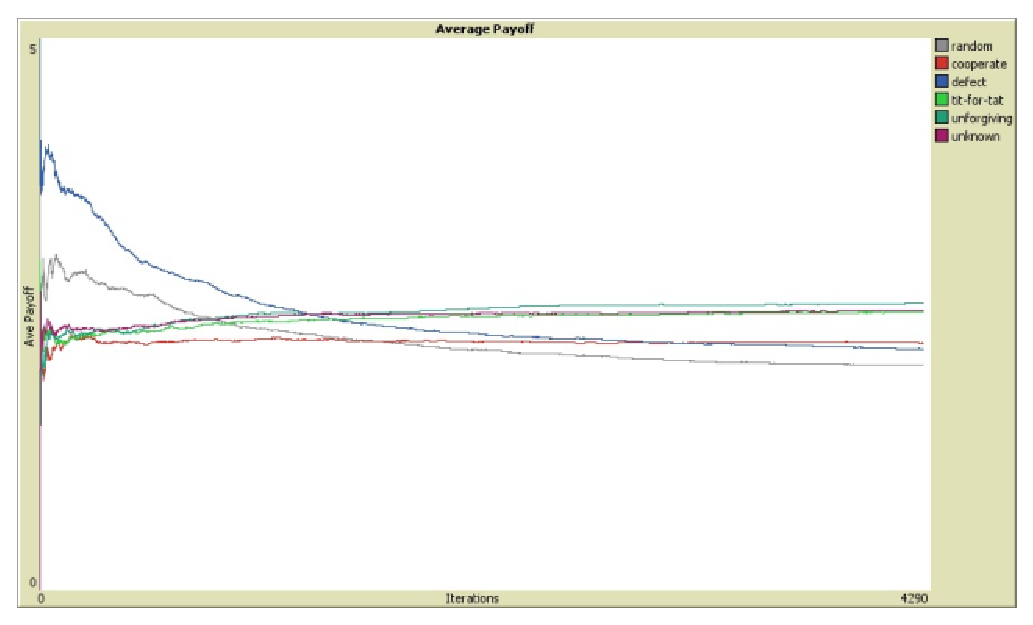
\includegraphics[width=13cm]{all10turtles-jpg.eps}
  \caption{All 10 strategies simulated with 10 turtles}
  \label{fig:all10turtles-jpg}
\end{figure}


\begin{figure}[!h]
  \centering
  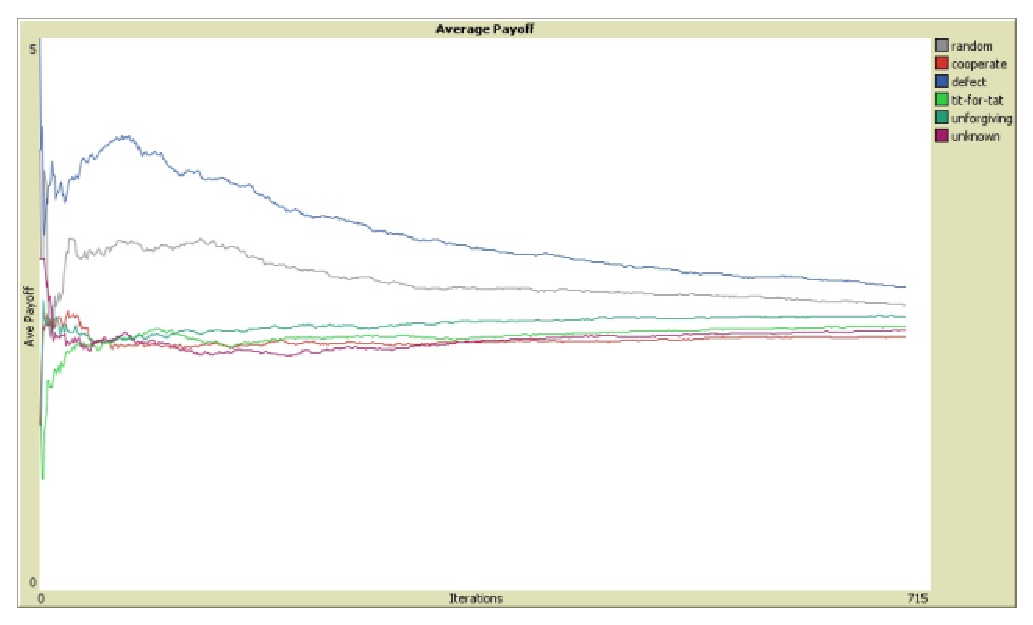
\includegraphics[width=13cm]{all10turtles_start-jpg.eps}
  \caption{First iterations of the simulations}
  \label{fig:all10turtles_start-jpg}
\end{figure}
This shows which strategy is the best for a short interaction with other nodes. Giving the largest pay-off in the beginning of the iterations. 

\begin{figure}[!h]
  \centering
  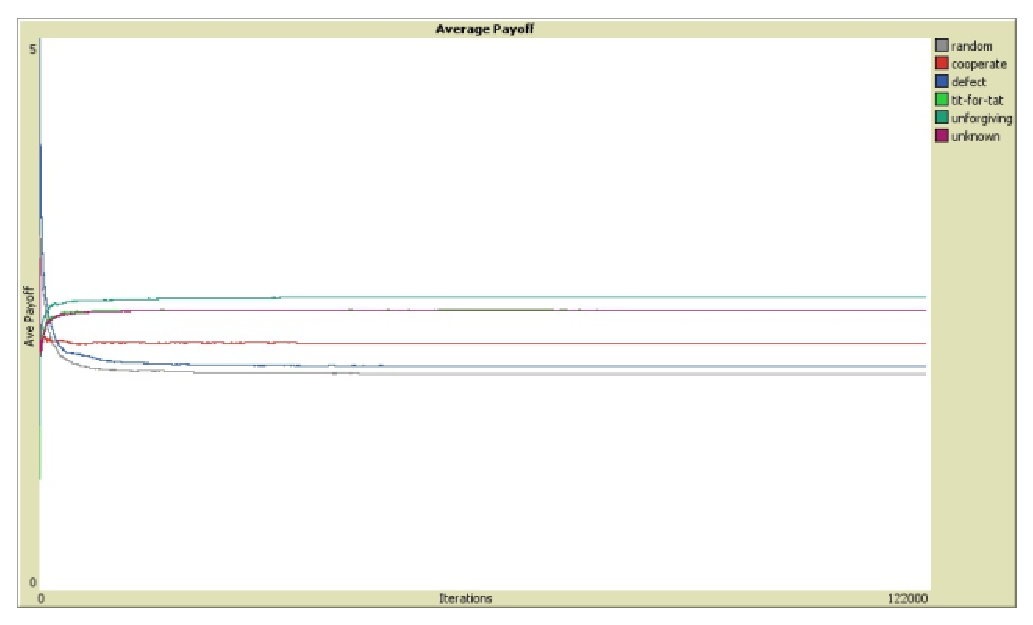
\includegraphics[width=13cm]{all10turtles_end-jpg.eps}
  \caption{Settling effect of the simulation}
  \label{fig:all10turtles_end-jpg}
\end{figure}
\FloatBarrier

The different strategies settles at the following pay-off rate:
\begin{pitemize}
	\item Random = 1.957
	\item Unforgiving = 2.657
	\item Unknown = 2.532
	\item Defect = 2.026
	\item Cooperate = 2.234
	\item Tit for Tat = 2.534
\end{pitemize}

Form these simulations and the just shown pay-off rates after settling it is possible to choose the best fitting strategy for a given scenario. It can be found that the unforgiving strategy is showing best results in the long run and that the defect strategy gives the best start pay-off. 
\newpage 